
JacORB implements a subset of the QoS policies defined in chapter
22.2 of the CORBA 3.0 specification.  In the following, we describe
each of the policies we have currently implemented, along with notes
on particular JacORB issues concerning each policy.  Policies not
listed in the following are not yet implemented.

As of yet, all policies described in this chapter are
\emph{client-side override policies}. The CORBA specification uses the
term for any policy that is explicitly set and thus overrides system
defaults. Policies can be set at different scopes: per object, per
thread, or per ORB. The current JacORB implementation only supports
object and ORB scopes. In general, the following steps are necessary: 

\begin{description}
\item[Step 1.] Get an {\tt any} from the ORB and put the value for the
           policy into it.
\item[Step 2.] Get a Policy object from the ORB which encapsulates the
           desired value (the {\tt any} value from the previous step).
\item[Step 3.]  Apply the policy to a particular object using the 
           {\tt \_set\_policy\_override()} operation on the object
           reference. 
\item[Step 3.] alternatively: set the policy ORB-wide using the {\tt
           set\_policy\_overrides()} operation on the ORB's
           {\tt PolicyManager} object.
\end{description}

Below is the code that corresponds to the steps listed above, using the
\emph{SyncScopePolicy} (described in the following section) as an
example. Also, have a look at the demo program in {\tt demo/policies}:

\begin{verbatim}
SomeCorbaType     server = ...
org.omg.CORBA.ORB orb    = ...
org.omg.CORBA.Any a      = orb.create_any();
a.insert_short(SYNC_WITH_SERVER.value); // the value for that policy
try
{
    Policy p = orb.create_policy(SYNC_SCOPE_POLICY_TYPE.value, a);
    server._set_policy_override (new Policy[]{ p },
                                 SetOverrideType.ADD_OVERRIDE);
    
    // get the ORB's policy manager
    PolicyManager policyManager = 
        PolicyManagerHelper.narrow( 
            orb.resolve_initial_references("ORBPolicyManager"));
    
    // set an ORB-wide policy
    policyManager.set_policy_overrides( new Policy[]{ p }, 
                                        SetOverrideType.ADD_OVERRIDE);
}
catch (PolicyError e)
{
    throw new RuntimeException ("policy error: " + e);
}
\end{verbatim}

The above is portable code that relies only on standardized CORBA APIs
to create and set policies.  Because this code is somewhat cumbersome
to write, JacORB also allows you to simplify it by creating the Policy
object directly via its constructor, as shown below. Note that this is
non-portable code:

\begin{verbatim}
SomeCorbaType server  = ...

Policy p = new org.jacorb.orb.policies.SyncScopePolicy
                                  (SYNC_WITH_TARGET.value);
server._set_policy_override (new Policy[]{ p },
                             SetOverrideType.ADD_OVERRIDE);
\end{verbatim}

See the package org.jacorb.orb.policies to find out which
constructors are defined for the individual policy types.

\section{Sync Scope}

The \emph{SyncScopePolicy} specifies at which point a oneway
invocation returns to the caller.  (The policy is ignored for
non-oneway invocations.)  There are four possible
values:

\begin{description}
\item[SYNC\_NONE] The invocation returns immediately.
\item[SYNC\_WITH\_TRANSPORT] The invocation returns after the request
  has been passed to the transport layer.
\item[SYNC\_WITH\_SERVER] The server sends an
  acknowledgement back to the client when it has received the
  request, but \emph{before} actually invoking the target.  The
  client-side call blocks until this acknowledgement has been
  received.
\item[SYNC\_WITH\_TARGET] An ordinary reply is sent back by the
  server, \emph{after} the target invocation has completed.  The
  client-side call blocks until this reply has been received.
\end{description}

The default mechanism in JacORB is \emph{SYNC\_WITH\_TRANSPORT},
since the call to the socket layer is a synchronous one.  In order to
implement \emph{SYNC\_NONE}, an additional thread is created on the
fly which in turn calls the socket layer, while the client-side
invocation returns after this thread has been created.  Given this
additional overhead, it is unlikely that \emph{SYNC\_NONE} yields a
significant performance gain for the client, not even on a
multiprocessor machine.

\section{Timing Policies}

For each CORBA request four different points in time can be specified:

\begin{description}
\item[Request Start Time] the time after which the request may be
  delivered to its target
\item[Request End Time] the time after which the request may no longer
  be delivered to its target
\item[Reply Start Time] the time after which the reply may be delivered
  to the client
\item[Reply End Time] the time after which the reply may no longer be
  delivered to the client
\end{description}

Each of these points in time can be specified on a per-object level as
a client-side override policy: \mbox{\emph{RequestStartTimePolicy}},
\emph{RequestEndTimePolicy}, \emph{ReplyStartTimePolicy}, and
\emph{ReplyEndTimePolicy} (see below for concrete code examples).

Each of these policies specifies an absolute time, which means that
they will usually have to be set again for each individual
request.  As a convenience, there are two additional policies that
allow you to specify a \emph{relative} time for \emph{Request End
Time} and \emph{Reply End Time}; they are called
\emph{RelativeRequestTimeoutPolicy} and
\emph{RelativeRoundtripTimeoutPolicy}, respectively.  These timeouts
are simply more convenient ways for expressing these two times;
before each individual invocation, the ORB computes absolute times
from them (measured from the start of the invocation at the client
side) and handles them just as if an absolute \emph{Request End Time}
or \emph{Reply End Time} had been specified.  We will therefore only
discuss the four absolute timing policies below.

All of these policies apply to synchronous and asynchronous
invocations alike.

\begin{figure}[htb]
  \begin{center}
    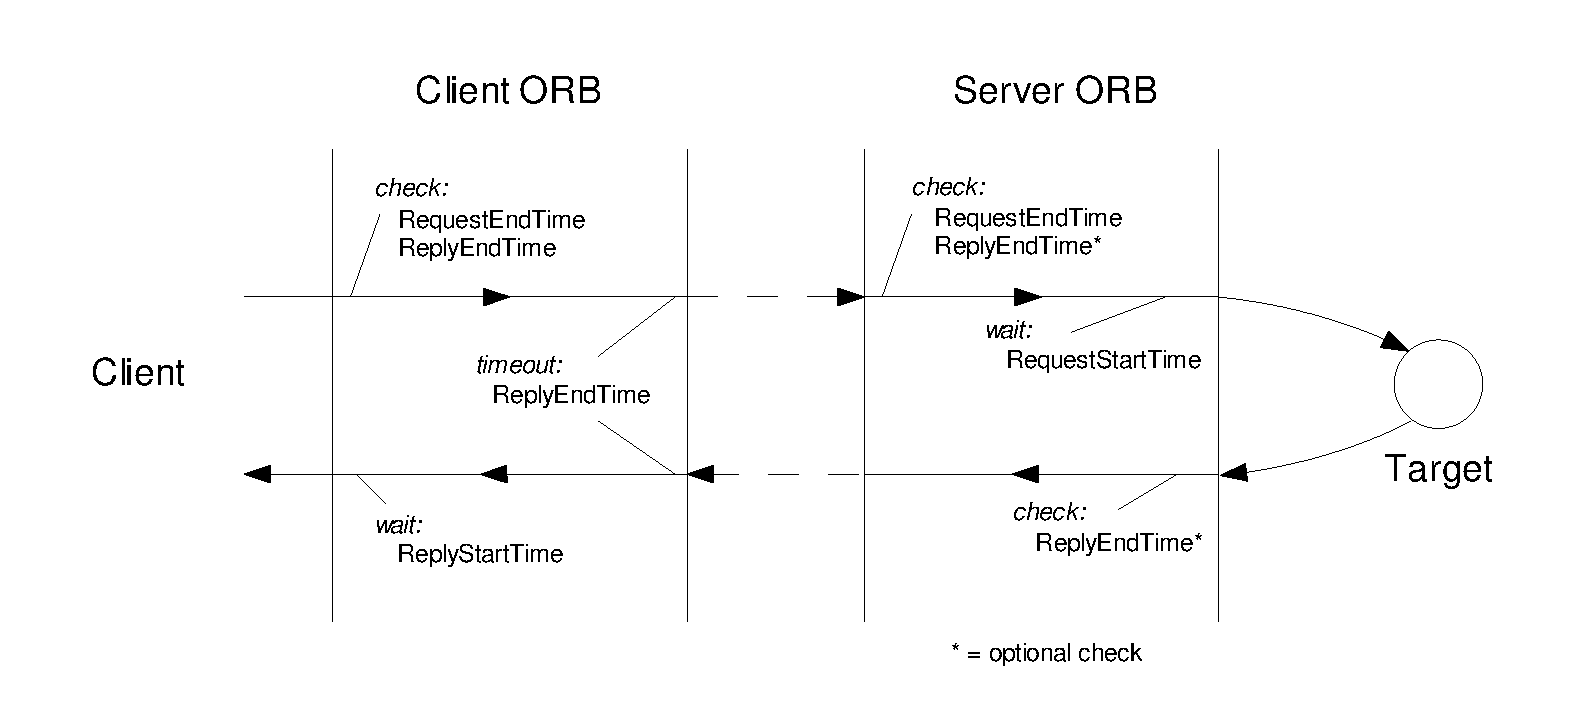
\includegraphics[width=16cm]{QoS/Timing}
  \end{center}
\caption{Timing Policies in JacORB}
\label{fig:timing}
\end{figure}

Figure \ref{fig:timing} shows how JacORB interprets the timing
policies in the course of a single request.

\begin{itemize}
\item As soon as the ORB receives control (prior to marshaling), it
converts any \emph{RelativeRequestTimeoutPolicy} or
\emph{RelativeRoundtripTimeoutPolicy} to an absolute value, by adding
the relative value to the current system time.

\item The ORB then checks whether \emph{Request End Time} or
\emph{Reply End Time} have already elapsed.  If so, no invocation is
made, and an {\tt org.omg.CORBA.TIMEOUT} is thrown to the client.

\item After the ORB has sent the request, it waits for a reply until
\emph{Reply End Time} has elapsed.  If it receives no reply before
that, the request is discarded and an {\tt org.omg.CORBA.TIMEOUT}
thrown to the client.  (JacORB does not currently cancel the
outstanding request, it simply discards the reply, should one arrive
after the timeout has elapsed.)\footnote{Note that if there is no
  connection to the server yet, other timeouts are applied first,
configured by the properties {\tt
  jacorb.connection.client.connect\_timeout} and {\tt
  jacorb.retries}.  If connection establishment fails, control does
not return to the client until these timeouts have expired, even if
this is later than \emph{Reply End Time}.}

\item On the server side (before demarshaling), the ORB checks whether
the \emph{Request End Time} has already elapsed.  If so, the request
is not delivered to the target, and an {\tt org.omg.CORBA.TIMEOUT}
is thrown back to the client.

\item Optionally, the server-side ORB may also check at this point
whether the \emph{Reply End Time} has already elapsed, and not
actually invoke the target in this case (throwing back an {\tt
org.omg.CORBA.TIMEOUT} to the client as well).  Since the \emph{Reply
  End Time} would then be checked both on the client and the server
side, this requires that the clocks on both machines are synchronized
at least to the same order of magnitude as the timeout itself.  This
check is therefore off by default, and may be enabled by setting the
property {\tt jacorb.poa.check\_reply\_end\_time} to ``on''.

\item If the request proceeds, the ORB waits until the \emph{Request
Start Time} has been reached, if one was specified, and has not
already elapsed.  After that, the request is delivered to the target.

\item After the target invocation has returned, the ORB may
optionally check whether the \emph{Reply End Time} has now elapsed.
Similar to the check prior to the target invocation, this check is
also optional and controlled by the property {\tt
jacorb.poa.check\_reply\_end\_time} (see discussion above).  If
the check is enabled, and the \emph{Reply End Time} is found to have
elapsed at this point, the ORB sends an {\tt org.omg.CORBA.TIMEOUT}
back to the client, rather than the actual reply.

\item If the reply arrives at the client before \emph{Reply End Time}
has elapsed, the ORB waits until \emph{Reply Start Time} has been
reached, if one was specified, and has not already elapsed.  After
that, the reply is delivered back to the client.

\end{itemize}

The bottom line of this is that for a simple, per-invocation timeout,
you should specify a \mbox{\emph{RelativeRoundtripTimeoutPolicy}}.

\clearpage{}
\subsection*{Programming}

In CORBA, points of time are specified to an accuracy of 100~nanoseconds, using
values of struct {\tt TimeBase::UtcT}.  To allow easy manipulation of such
values from Java, JacORB provides a number of static methods in {\tt
org.jacorb.util.Time}.  For example, to convert the current Java time
into a {\tt UtcT} value, write

\begin{verbatim}
UtcT currentTime = org.jacorb.util.Time.corbaTime();
\end{verbatim}

To create a {\tt UtcT} value that specifies a time $n$~milliseconds in the
future, you can write

\begin{verbatim}
UtcT time = org.jacorb.util.Time.corbaFuture (10000 * n);
\end{verbatim}

(The argument to {\tt corbaFuture()} is in CORBA time units of
100~ns; we multiply $n$ by 10000 here to convert it from Java time
units (milliseconds).)

The following shows how to set a timing policy for an object using the
standard mechanism (see the beginning of this chapter for an
explanation).  In this example, we set a \emph{Reply End Time} that
lies one second in the future:

\begin{verbatim}
import org.omg.CORBA.*;

SomeCorbaType server  = ...  // the object for which we want to set
                             // a timing policy
org.omg.CORBA.ORB orb = ...
org.omg.CORBA.Any a   = orb.create_any();

org.omg.TimeBase.UtcT replyEndTime
    = org.jacorb.util.Time.corbaFuture (1000 * 10000);  // one second

org.omg.TimeBase.UtcTHelper.insert (a, replyEndTime);

try
{
    Policy p
        = orb.create_policy (REPLY_END_TIME_POLICY_TYPE.value, a);
    server._set_policy_override (new Policy[]{ p },
                                 SetOverrideType.ADD_OVERRIDE);
}
catch (PolicyError e)
{
    ...
}
\end{verbatim}

\clearpage{}

Using the constructors of JacORB's implementations of policy values,
this becomes less verbose:

\begin{verbatim}
SomeCorbaType server  = ...

Policy p = new org.jacorb.orb.policies.ReplyEndTimePolicy
                   (org.jacorb.util.Time.corbaFuture (1000 * 10000));

server._set_policy_override (new Policy[]{ p },
                             SetOverrideType.ADD_OVERRIDE);
\end{verbatim}

Likewise, to set a \emph{Relative Roundtrip Timeout} of one second,
write:

\begin{verbatim}
SomeCorbaType server  = ...

Policy p =
    new org.jacorb.orb.policies.RelativeRoundtripTimeoutPolicy 
                                                      (1000 * 10000);

server._set_policy_override (new Policy[]{ p },
                             SetOverrideType.ADD_OVERRIDE);
\end{verbatim}

The difference between this and the example before, where a
\emph{Reply End Time} was used, is that the latter specifies a
\emph{relative time} to CORBA.  The policy will therefore be valid
for all subsequent invocations, because the absolute deadline will be
recomputed before each invocation.  In the first example, the
deadline will no longer make sense for any subsequent invocations,
since only an absolute time was specified to the ORB.


%%% Local Variables: 
%%% mode: latex
%%% TeX-master: "../ProgrammingGuide"
%%% End: 
